\chapter{Graphic Models}
To compute $P(x_1,...,x_d)$, we can utilize the chain rule $P(x_1,...,x_d)=P(x_1)\prod_{i=2}^d P(x_i|x_{1:i-1})$. However, this approach becomes computationally expensive as the dimension $d$ increases.

Fortunately, when there are conditionally independent relationships between variables, such as $x_A \bot x_C | x_B$, we can reduce the computational cost.

In this section, we can employ graphical models to represent probabilistic relationships between variables, particularly when there are conditionally independent relationships present.
\section{Graph Theory}
\begin{enumerate}
    \item A graph $(V,E)$, $V$ is a set of \textit{vertices}, $E\subseteq V\times V$ is a set of ordered pairs of vertices, called \textit{edges}.
    
    An edge $(i,j)\in E$ is \textit{directed} if $(i,j)\notin E$; otherwise the edge is \textit{undirected}. We denote directed and undirected edges by the symbols $i \rightarrow j$ and $i\sim j$, respectively.
    \item \textbf{Directed and Undirected Graphs:} Graphs in which \textit{all} edges are directed (resp. undirected).
    \item \textbf{Subgraph:} a subgraph $(S,E_S)$ of $(V,E)$ is a subset $S\subset G$ with edges that have both endpoints in $S$.
    \item \textbf{Clique:} A set $C$ of vertices in an undirected graph is a \underline{clique} if either $C$ is a singleton, or \textbf{each pair of vertices in $C$ is linked by an edge}.\\
    That is, all vertices in $C$ are neighbors. The clique is \underline{maximal} if there is no larger clique that contains $C$.
    \item \textbf{Parent, Child:} Vertex $i$ is a \underline{parent} of vertex $j$ if $i \rightarrow j$, in which case $j$ is also called a \underline{child} of $i$. We denote by $\pi(j)$ the set of parents of $j$.
    \item \textbf{Path:} A \textit{path} of length $n$ from $i$ to $j$ is a sequence $i = k_0,k_1,...,k_n = j$ of distinct vertices such that ($k_{m-1},k_m) \in E$ for all $m = 1,... ,n$. We designate such a path by $i \rightarrow j$.
    \item \textbf{Connected Graph:} An undirected graph is \underline{connected} if there is a path between any pair of nodes. In general, the connected components of a graph are those subgraphs which are connected.
    \item \textbf{Cycle/Loop:} An $n-$cycle, or loop, is a path of length $n$ $i \rightarrow j$ with $i = j$.
    
    A directed graph without cycle is also called Directed Acyclic Graph (DAG)
    \item \textbf{Tree:} A tree is a connected, undirected graph without cycles; \textbf{it has a unique path between any two vertices}.
    \item \textbf{Rooted Tree:} A rooted tree is the directed acyclic graph obtained from a tree by choosing as vertex as root and directing all edges away from this root. Each vertex of a rooted tree has at most one parent.
    \item \textbf{Forest:} A forest is an undirected graph where all connected components are trees.
\end{enumerate}
\begin{center}\begin{figure}[htbp]
    \centering
    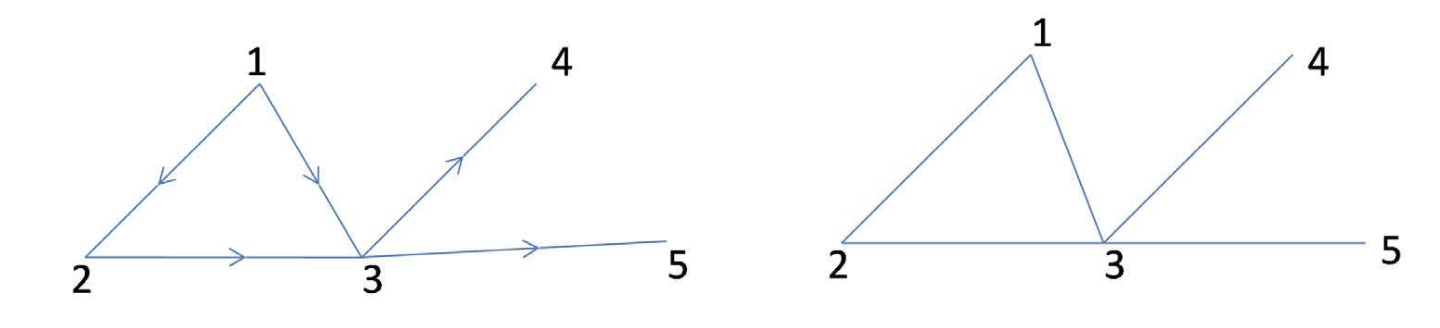
\includegraphics[scale=0.25]{graph.png}
    \caption{(a) Directed and (b) Undirected graph.}
    \label{}
\end{figure}\end{center}

\section{Bayesian Networks}
A Bayesian network (or belief network) is a joint probability distribution associated with a \textit{directed acyclic graph} $(V,E)$ whose nodes $X_v, v \in V$ are random variables. The joint distribution is of the form
\begin{equation}
    \begin{aligned}
        p(\vec{x})=\prod_{v\in V}p(x_v|\pi(x_v))
    \end{aligned}
    \nonumber
\end{equation}
$\pi(x_v)$ is the set of parents of vertices.

For instance a Markov chain is a chain-type directed acyclic graph where $V = \{1, 2,..., n\}$, and $\pi(v) = v - 1$ for $v \geq 2$. The pmf for the sequence $\vec{x}$ is obtained from the chain rule
\begin{equation}
    \begin{aligned}
        p(\vec{x})=p(x_1)p(x_2|x_1)\cdots p(x_n|x_{n-1})
    \end{aligned}
    \nonumber
\end{equation}

\section{Markov Networks}
\subsection{General Form}
We can use undirected graph to represent conditionally independent.
\begin{center}\begin{figure}[htbp]
    \centering
    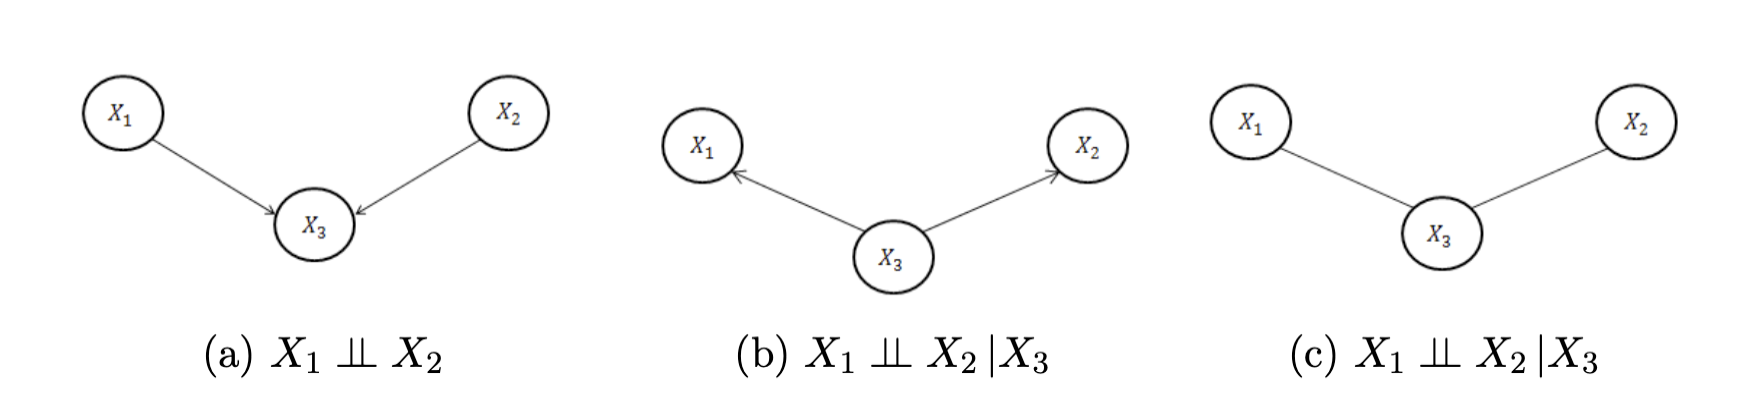
\includegraphics[scale=0.2]{BM.png}
    \caption{(a) (b) Two Bayesian networks and (c) a Markov network.}
    \label{}
\end{figure}\end{center}
More generally, if two nodes $X_u$ and $X_v$ in a Markov network are not connected by an edge, then the random variables $X_u$ and $X_v$ are conditionally independent given all the other random variables (denoted by $X_u \perp X_v \mid X_{\mathcal{V} \backslash\{u, v\}}$).

A Markov network is an undirected graph $G = (V,E)$ together with a collection $X = \{X_v, v \in V\}$ of random variables indexed by the nodes of $G$.

Since there is no direction, we use \textbf{clique} to help use represent probabilities. (\textit{Review: \underline{clique} is a set of vertices that each pair of vertices is linked})

We use $\Omega$ let be collection of cliques in the graph and the functions $\psi_C(\cdot)$ be the \textbf{\textit{clique potentials}, or \textit{compatibility functions}}.

The pmf of $X$ takes the form
\begin{equation}
    \begin{aligned}
        p(\vec{x})=\frac{\prod_{C\in \Omega}\psi_C(\vec{x}_C)}{\sum_{\vec{x}}\prod_{C}\psi_C(\vec{x}_C)}=\frac{1}{Z}\prod_{C\in \Omega}\psi_C(\vec{x}_C)
    \end{aligned}
    \nonumber
\end{equation}
where $Z=\sum_{\vec{x}}\prod_{C}\psi_C(\vec{x}_C)$ is a normalization constant.

\textbf{Note:} this is a form of factorization that can represent conditionally independent relationship among variables. $\psi_C(\cdot)$ are undefined functions.x

\subsection{Hammersley-Clifford theorem}
\begin{theorem}[Hammersley-Clifford theorem]
    Assume that $p\left(x_1, \ldots, x_n\right)>0$ (positivity condition). Then,
    $$
    p(\vec{x})=\frac{1}{Z} \prod_{\substack{C \in \Omega}} \phi_C\left(\vec{x}_C\right)
    $$
    Thus, the following are equivalent (given the positivity condition):
    \begin{enumerate}
        \item \textbf{Local Markov property:} $p\left(x_i \mid \vec{x} \backslash\left\{x_i\right\}\right)=p\left(x_i \mid \mathcal{N}\left(x_i\right)\right)$, where $\mathcal{N}\left(x_i\right)$ is the neighboring set of $x_i$.
        \item \textbf{Factorization property:} The probability factorizes according
        to the cliques of the graph.
        \item \textbf{Global Markov property:} $p\left(\vec{x}_A \mid \vec{x}_B, \vec{x}_S\right)=p\left(\vec{x}_A \mid \vec{x}_S\right)$
        whenever $\vec{x}_A$ and $\vec{x}_B$ are separated by $\vec{x}_S$ in $G$
    \end{enumerate}
\end{theorem}

\subsection{Form of Gibbs distribution (Boltzmann distribution)}
The factorization is not unique.
We let $\psi(\vec{x}_C)=e^{-V_C(\vec{x}_C)}$, where $V_C(\cdot)$ are the so-called potential energy functions. In a pairwise Markov network, $p(\vec{x})$ can be expressed as a product of clique potentials involving either one or two random variables.
\begin{equation}
    \begin{aligned}
        p(\vec{x})=\frac{1}{Z}e^{-\sum_CV_C(x_C)}
    \end{aligned}
    \nonumber
\end{equation}
This probability follows \textbf{Gibbs distribution (Boltzmann distribution)}. This distribution follows exponential families.

\section{Conversion of directed graph to undirected graph}
We can use a step known as \textit{moralization}.
Moralization of graph: connect two unmarried parents.

This is the process of “marrying” the parents of each node, i.e., adding an edge connecting any pair of parents if one did not exist. The figure illustrates this process for a node with three parents. In this case the undirected graph consists of a clique of size 4.
\begin{center}\begin{figure}[htbp]
    \centering
    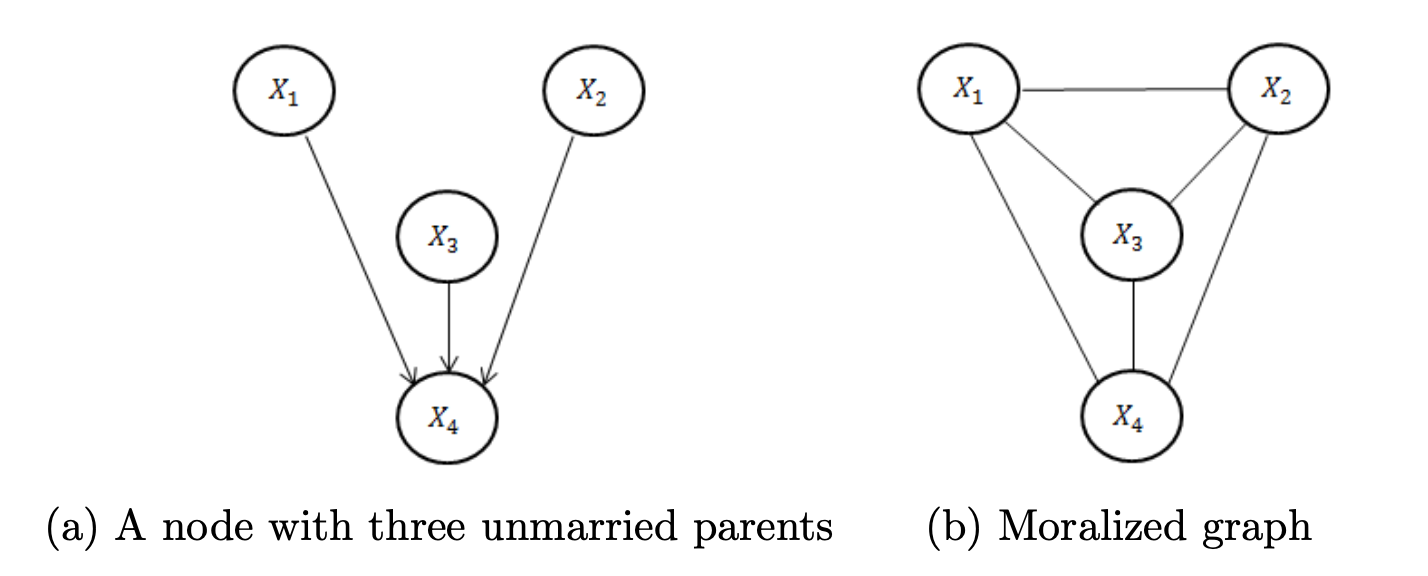
\includegraphics[scale=0.25]{moralization.png}
    \caption{Graph moralization}
    \label{}
\end{figure}\end{center}

\section{ Inference and Learning}
\subsection{Inference on Trees}
Consider the tree of the figure, which has 5 nodes and edges $1\sim 2\sim 3$ and $4\sim 3\sim 5$. We have
\begin{equation}
    \begin{aligned}
        p(\vec{x})=\frac{1}{Z}\psi_{12}(x_1,x_2)\psi_{23}(x_2,x_3)\psi_{34}(x_3,x_4)\psi_{35}(x_3,x_5)
    \end{aligned}
    \nonumber
\end{equation}
\begin{center}\begin{figure}[htbp]
    \centering
    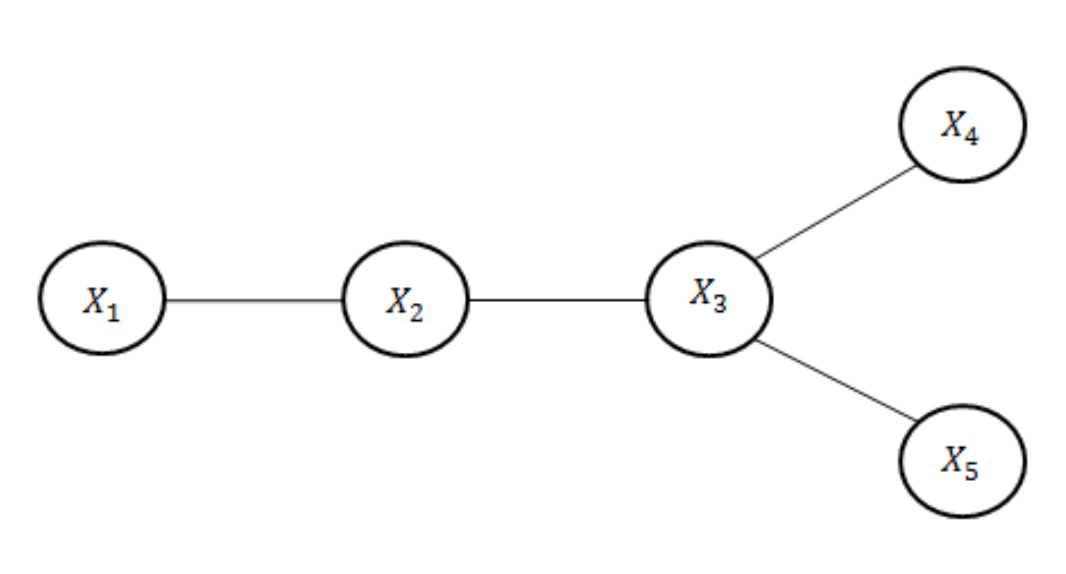
\includegraphics[scale=0.2]{inftree.png}
    \caption{Example 1}
    \label{}
\end{figure}\end{center}
\begin{enumerate}
    \item \textbf{Marginal Inference:} As a first example of inference on trees, consider the problem of evaluating the marginal pmf $p(x_5)$. We explore two approaches: the \textbf{direct approach}, which is computationally infeasible for large graphs (the number of items in the sum is $|\mathcal{X}|^4$);
    $$p(x_5)=\sum_{x_1,...,x_4}\frac{1}{Z}\psi_{12}(x_1,x_2)\psi_{23}(x_2,x_3)\psi_{34}(x_3,x_4)\psi_{35}(x_3,x_5)$$
    and the \textbf{sum-product algorithm}, which exploits the graph structure.
    $$
    \begin{aligned}
    p\left(x_5\right) &=\frac{1}{Z} \sum_{x_3} \psi_{35}\left(x_3, x_5\right) \sum_{x_4} \psi_{34}\left(x_3, x_4\right) \sum_{x_2} \psi_{23}\left(x_2, x_3\right) \underbrace{\sum_{x_1} \psi_{12}\left(x_1, x_2\right)}_{m_{1 \rightarrow 2}\left(x_2\right)} \\
    &=\frac{1}{Z} \sum_{x_3} \psi_{35}\left(x_3, x_5\right) \sum_{x_4} \psi_{34}\left(x_3, x_4\right) \underbrace{\sum_{x_2} \psi_{23}\left(x_2, x_3\right) m_{1 \rightarrow 2}\left(x_2\right)}_{m_{2 \rightarrow 3}\left(x_3\right)} \\
    &=\frac{1}{Z} \sum_{x_3} \psi_{35}\left(x_3, x_5\right) m_{2 \rightarrow 3}\left(x_3\right) \underbrace{\sum_{x_4} \psi_{34}\left(x_3, x_4\right)}_{m_{4 \rightarrow 3}\left(x_3\right)} \\
    &=\frac{1}{Z} \underbrace{\sum_{x_3} \psi_{35}\left(x_3, x_5\right) m_{2 \rightarrow 3}\left(x_3\right) m_{4 \rightarrow 3}\left(x_3\right)}_{m_{3 \rightarrow 5}\left(x_5\right)} .
    \end{aligned}
    $$
    In this derivation, nodes $1,2,4,3$ are eliminated in that order. We think of each term $m_{i \rightarrow j}\left(x_j\right)$ as a message conveyed from node $i$ to node $j$, just before elimination of $j$. Computing $m_{i \rightarrow j}\left(x_j\right)$ involves a summation over all possible values of $x_i$. This interpretation will be helpful in more complex problems.
    \begin{center}\begin{figure}[htbp]
        \centering
        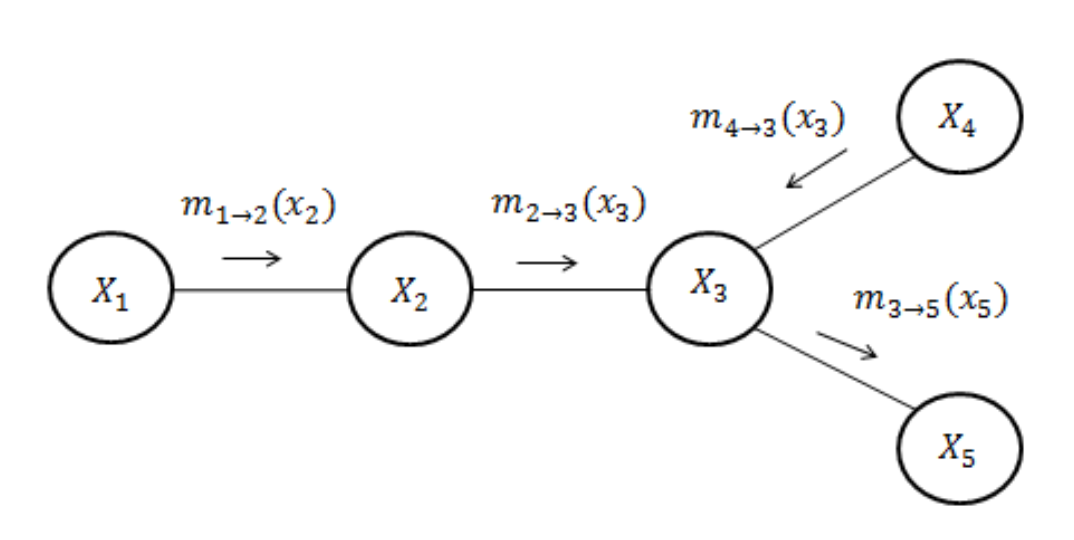
\includegraphics[scale=0.2]{belief.png}
        \caption{Belief propagation in a tree}
        \label{}
    \end{figure}\end{center}
    As illustrated in the Figure, a node can send a message to a neighbor once it has received messages from all of its other neighbors. For a general tree, upon choosing an elimination order, we evaluate the following messages in the corresponding order:
    $$
    m_{i \rightarrow j}\left(x_j\right)=\sum_{x_i} \psi_{i j}\left(x_i, x_j\right) \prod_{k \in \mathcal{N}(i) \backslash\{j\}} m_{k \rightarrow i}\left(x_i\right)
    $$
    The marginal probability at any node $i$ is the product of all incoming messages:
    $$
    p\left(x_i\right)=\frac{1}{Z} \prod_{k \in \mathcal{N}(i)} m_{k \rightarrow i}\left(x_i\right) .
    $$
    We can also evaluate the 2D marginal $p(x_2,x_5)$
    $$
    p\left(x_2, x_5\right)=\frac{1}{Z} \sum_{x_3} \psi_{23}\left(x_2, x_3\right) \psi_{35}\left(x_3, x_5\right) \underbrace{\sum_{x_4} \psi_{34}\left(x_3, x_4\right)}_{m_{4 \rightarrow 3}\left(x_3\right)} \underbrace{\sum_{x_1} \psi_{12}\left(x_1, x_2\right)}_{m_{1 \rightarrow 2}\left(x_2\right)} .
    $$
    Finally, a conditional marginal such as $p\left(x_1 \mid x_5\right)$ is obtained as $p\left(x_1, x_5\right) / p\left(x_5\right)$, hence the problem is reduced to evaluating unconditional marginals.

    The computational cost of the algorithm is $O\left(n|\mathcal{X}|^2\right)$ when the $n$ random variables are defined over the same alphabet $\mathcal{X}$.

    \item \textbf{Maximization:} A closely related problem is to find the most likely configuration, possibly by fixing some coordinates. For instance, evaluate
    $$
    M\left(x_5\right)=\max _{x_1, x_2, x_3, x_4} p\left(x_1, x_2, x_3, x_4, x_5\right)
    $$
    for the above Markov network. Direct calculation has exponential complexity. However, the more efficient max-product algorithm has the same structure as the sum-product algorithm:
    \begin{equation}
        \begin{aligned}
            M\left(x_5\right)&=\max _{x_1, x_2, x_3, x_4} \frac{1}{Z} \psi_{12}\left(x_1, x_2\right) \psi_{23}\left(x_2, x_3\right) \psi_{34}\left(x_3, x_4\right) \psi_{35}\left(x_3, x_5\right)\\
            &=\frac{1}{Z} \max _{x_3} \psi_{35}\left(x_3, x_5\right) \max _{x_4} \psi_{34}\left(x_3, x_4\right) \max _{x_2} \psi_{23}\left(x_2, x_3\right) \underbrace{\max _{x_1} \psi_{12}\left(x_1, x_2\right)}_{m_{1 \rightarrow 2}\left(x_2\right)}\\
            &=\frac{1}{Z} \max _{x_3} \psi_{35}\left(x_3, x_5\right) \underbrace{\max _{x_4} \psi_{34}\left(x_3, x_4\right)}_{m_{4 \rightarrow 3}\left(x_3\right)} \underbrace{m_{x_2} \psi_{23}\left(x_2, x_3\right) m_{1 \rightarrow 2}\left(x_2\right)}_{m_{2 \rightarrow 3}\left(x_3\right)}\\
            &=\frac{1}{Z} \underbrace{\max _{x_3} \psi_{35}\left(x_3, x_5\right) m_{4 \rightarrow 3}\left(x_3\right) m_{2 \rightarrow 3}\left(x_3\right)}_{m_{3 \rightarrow 5}\left(x_5\right)}
        \end{aligned}
        \nonumber
    \end{equation}
\end{enumerate}

